\documentclass[letterpaper,9pt,twocolumn,twoside,]{pinp}

%% Some pieces required from the pandoc template
\providecommand{\tightlist}{%
  \setlength{\itemsep}{0pt}\setlength{\parskip}{0pt}}

% Use the lineno option to display guide line numbers if required.
% Note that the use of elements such as single-column equations
% may affect the guide line number alignment.

\usepackage[T1]{fontenc}
\usepackage[utf8]{inputenc}

% pinp change: the geometry package layout settings need to be set here, not in pinp.cls
\geometry{layoutsize={0.95588\paperwidth,0.98864\paperheight},%
  layouthoffset=0.02206\paperwidth, layoutvoffset=0.00568\paperheight}

\definecolor{pinpblue}{HTML}{185FAF}  % imagecolorpicker on blue for new R logo
\definecolor{pnasbluetext}{RGB}{101,0,0} %



\title{Abalone Dataset}

\author[]{Group\_Early\_5}

  \affil[]{SID1,SID2,490443251,490209370,490384806}

\setcounter{secnumdepth}{0}

% Please give the surname of the lead author for the running footer
\leadauthor{Author and Author}

% Keywords are not mandatory, but authors are strongly encouraged to provide them. If provided, please include two to five keywords, separated by the pipe symbol, e.g:
 \keywords{  one |  two |  optional |  keywords |  here  }  

\begin{abstract}
We are doing multiple regression on an abalone dataset with 4177
observations with 9 different variables to see if we could use several
physical measurements to predict the rings of abalones,which gives us
the ages of abalones in years.In order to select an appropriate model,
we did some log transformation and square root of transformations to
appropriately fit the observed values into model.In addition to that we
ran forward and backward approach in distinguishing the most appropriate
model and finally interpret the result from the model.
\end{abstract}

\dates{This version was compiled on \today} 


% initially we use doi so keep for backwards compatibility
% new name is doi_footer
\doifooter{\url{https://cran.r-project.org/package=YourPackage}}

\pinpfootercontents{YourPackage Vignette}

\begin{document}

% Optional adjustment to line up main text (after abstract) of first page with line numbers, when using both lineno and twocolumn options.
% You should only change this length when you've finalised the article contents.
\verticaladjustment{-2pt}

\maketitle
\thispagestyle{firststyle}
\ifthenelse{\boolean{shortarticle}}{\ifthenelse{\boolean{singlecolumn}}{\abscontentformatted}{\abscontent}}{}

% If your first paragraph (i.e. with the \dropcap) contains a list environment (quote, quotation, theorem, definition, enumerate, itemize...), the line after the list may have some extra indentation. If this is the case, add \parshape=0 to the end of the list environment.

\acknow{This template package builds upon, and extends, the work of the
excellent \href{https://cran.r-project.org/package=rticles}{rticles}
package, and both packages rely on the
\href{http://www.pnas.org/site/authors/latex.xhtml}{PNAS LaTeX} macros.
Both these sources are gratefully acknowledged as this work would not
have been possible without them. Our extensions are under the same
respective licensing term
(\href{https://www.gnu.org/licenses/gpl-3.0.en.html}{GPL-3} and
\href{https://www.latex-project.org/lppl/}{LPPL (\textgreater{}= 1.3)}).}

\subsection{Introduction}\label{introduction}

Use multiple regression to analyse a data set of abalones with multiple
predictor variables,namely whole weight,shuck weight,viscera
weight,shell weight,diameters,length,height of the abalones.

\subsection{Data set}\label{data-set}

The original data was collected by the Marine Resources Division in
Taroona, Tasmania. The current set is provided by the University of
California Irvine Machine Learning Repository. It contains 4177
observations with 8 different numerical variables, 1 categorical and no
missing value. 2 unwanted outliers were found in the height variable
which will be disregarded.

In detail, main variables that were analysed were physical attributes of
the abalone ranging from dimensions of the length, diameter of the
shell, the height of the abalone captured in millimeters and weighting
variables that encompass specific weights varying from the weight of the
meat, after bleeding to the weight of the shell captured in grams. After
some typing and data type corrections, Rings is the most relevant and
suitable variable to Age that is the variable to be predicted.

\subsection{Analysis}\label{analysis}

Assumptions: * Linearity:there's no obvious curvature in the residual vs
fitted values plot,looks linear enough. * Independence:the data was
independently collected over 5 different regions in the tasman sea as
the article about the dataset said. * Homoskedasticity: the residuals
don't appear to be fanning out or changing their variability over the
range of the fitted values.

\begin{itemize}
\tightlist
\item
  Normality:In the QQ plot, the points are reasonably close to the
  diagonal line,except for the trivial bottom 5 or so points.
\end{itemize}

\subsection{Results:}\label{results}

Investigation Question: Can we predict the number of rings abalones
have, using only an abalones physical attributes which are easily and
quickly measured?

\begin{itemize}
\tightlist
\item
  All variables have significant p-values giving evidence that there is
  a significant relationship between them and the square root log of the
  number of rings.
\item
  When we examine the significance of each level of our sex variable, we
  decided to retain the sex factor of whether abalones are infants or
  adults rather than whether abalones are male, female or infant due to
  how the p-value of sex\_female not providing enough evidence to reject
  the null hypothesis that coefficient is equal to zero. This is done by
  utilising stepping forward and stepping backwards AICs, we have
  arrived at two models with the same adjusted R\^{}2 thus we need to
  encompass the RMSE and MAE to identify the better performing model.
\end{itemize}

\textbf{Cross validation} was used to compute RMSE and MAE to account
for and minimise overfitting. RMSE and MAE values of the backward model
are slightly smaller compared to forward model's. Hence we proceed with
the backward model.

Therefore the following is our model,

Which can be translated into an equivalent model

\begin{equation}
  \begin{aligned}
\widehat{\sqrt{log(rings)}} = 1.45 + 0.20 log(whole)\\
       &- 0.19 log(shucked) - 0.02 log(viscera) \\
       &+ 0.11 log(shell) + 0.07 log(diameter)\\
       &- 0.08 log(length) + 0.12 \sqrt{height}\\
       &- 0.01 Sex_{infant}\\
  \end{aligned}
\end{equation}

\begin{equation}
  \begin{aligned}
\widehat{log(rings)} = 2.1025 + 0.08log(whole)\\
       &- 0.0722 log(shucked) - 0.0008log(viscera) \\
       &+ 0.0242 log(shell) + 0.0098log(diameter)\\
       &- 0.0128 log(length) + 0.0144(height)\\
       &- 0.0001 Sex_{infant}^2\\
  \end{aligned}
\end{equation}

On average a one percent increase in:

\begin{itemize}
\tightlist
\item
  Whole weight will result in a 0.08\% change in number of rings
\item
  Shucked weight will result in a 0.0722\% change in number of rings
\item
  Viscera weight will result in a 0.0008\% change in number of rings
\item
  Shell weight will result in a 0.0242\% change in number of rings
\item
  Diameter will result in a 0.0098\% change in number of rings
\item
  Length will result in a 0.0128\% change in number of rings
\end{itemize}

And on average, a one unit increase in:

\begin{itemize}
\tightlist
\item
  Height will result in a 0.0144 x 100\% change in number of rings
\item
  Sex\_infant will result in a 0.0001 x 100\% change in number of rings
\end{itemize}

\subsection{Discussion and conclusion:}\label{discussion-and-conclusion}

The PNAS sample included a fixed PNG image here, but this document
prefers to show the results and embedding of \emph{R} code.

\subsection{Digital Figures}\label{digital-figures}

\begin{figure*}
  \begin{center}
    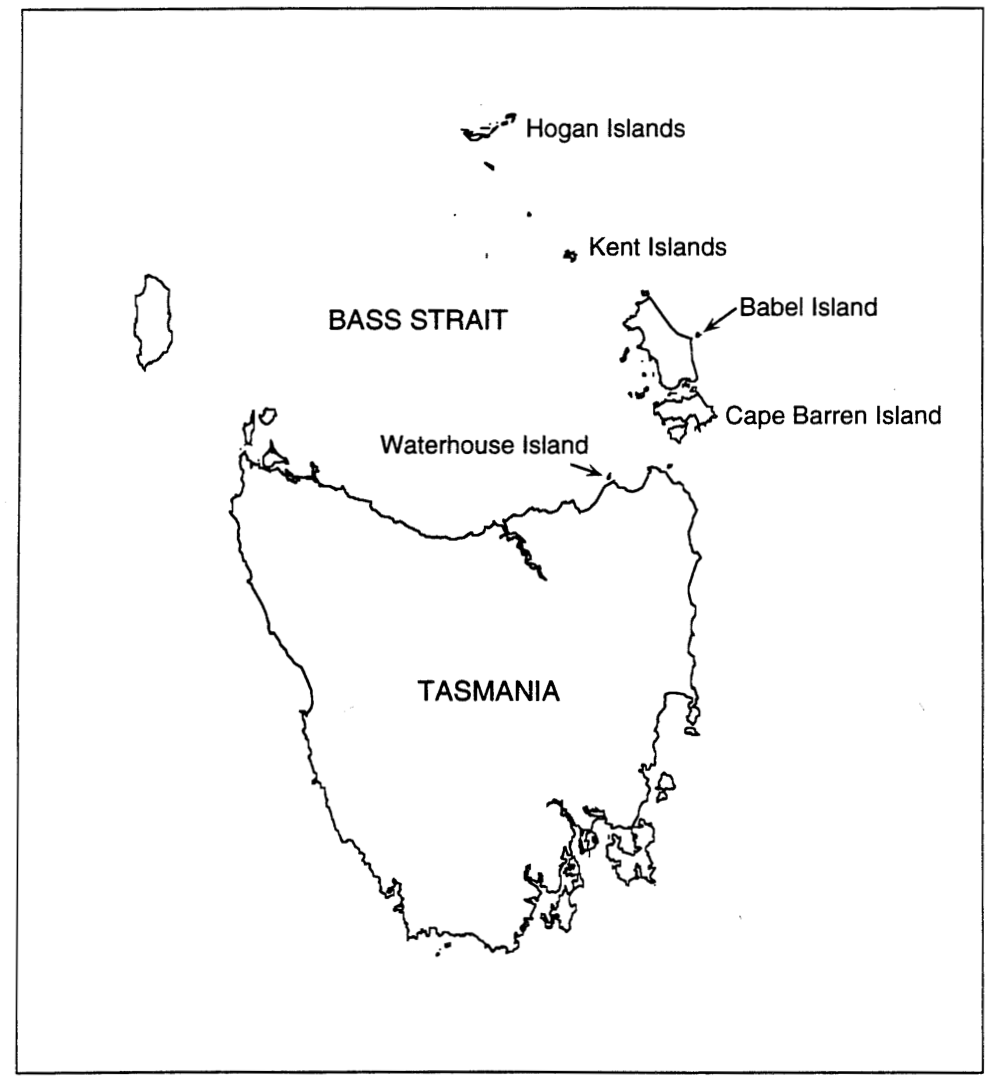
\includegraphics[width=0.66\textwidth, height=3.5in]{Independence} 
  \end{center}
  \caption{Wide ggplot2 figure}\label{fig}
\end{figure*}

\subsection{Typeset Code (But Do Not Run
It)}\label{typeset-code-but-do-not-run-it}

\subsection{Single column equations}\label{single-column-equations}

%\showmatmethods
\showacknow


\bibliography{pinp}
\bibliographystyle{jss}



\end{document}

